\section{Zielsetzung}
\label{sec:Zielsetzung}
In diesem Versuch sollen unbekannte Widerstände, Induktivitäten und Kapazitäten durch Brückenschaltungen ermittelt werden.
Darüber hinaus soll die Frequenzabhängigkeit der Brückenspannung einer Wien-Robinson-Brücke gemessen werden und eine Klirrfaktor-Messung durchgeführt werden.
\section{Theorie}
\label{sec:Theorie}
Mithilfe von Brückenschaltungen können physikalische Größen, die durch ohmsche, aber auch komplexe Widerstände darstellbar sind, gut gemessen werden.
Da die Genauigkeit der Messungen mit einer Nullmethode erhöht wird, werden diese mit abgeglichen Brücken durchgeführt.

\subsection{Allgemeiner Aufbau einer Brückenschaltung}
\begin{figure}
    \centering
    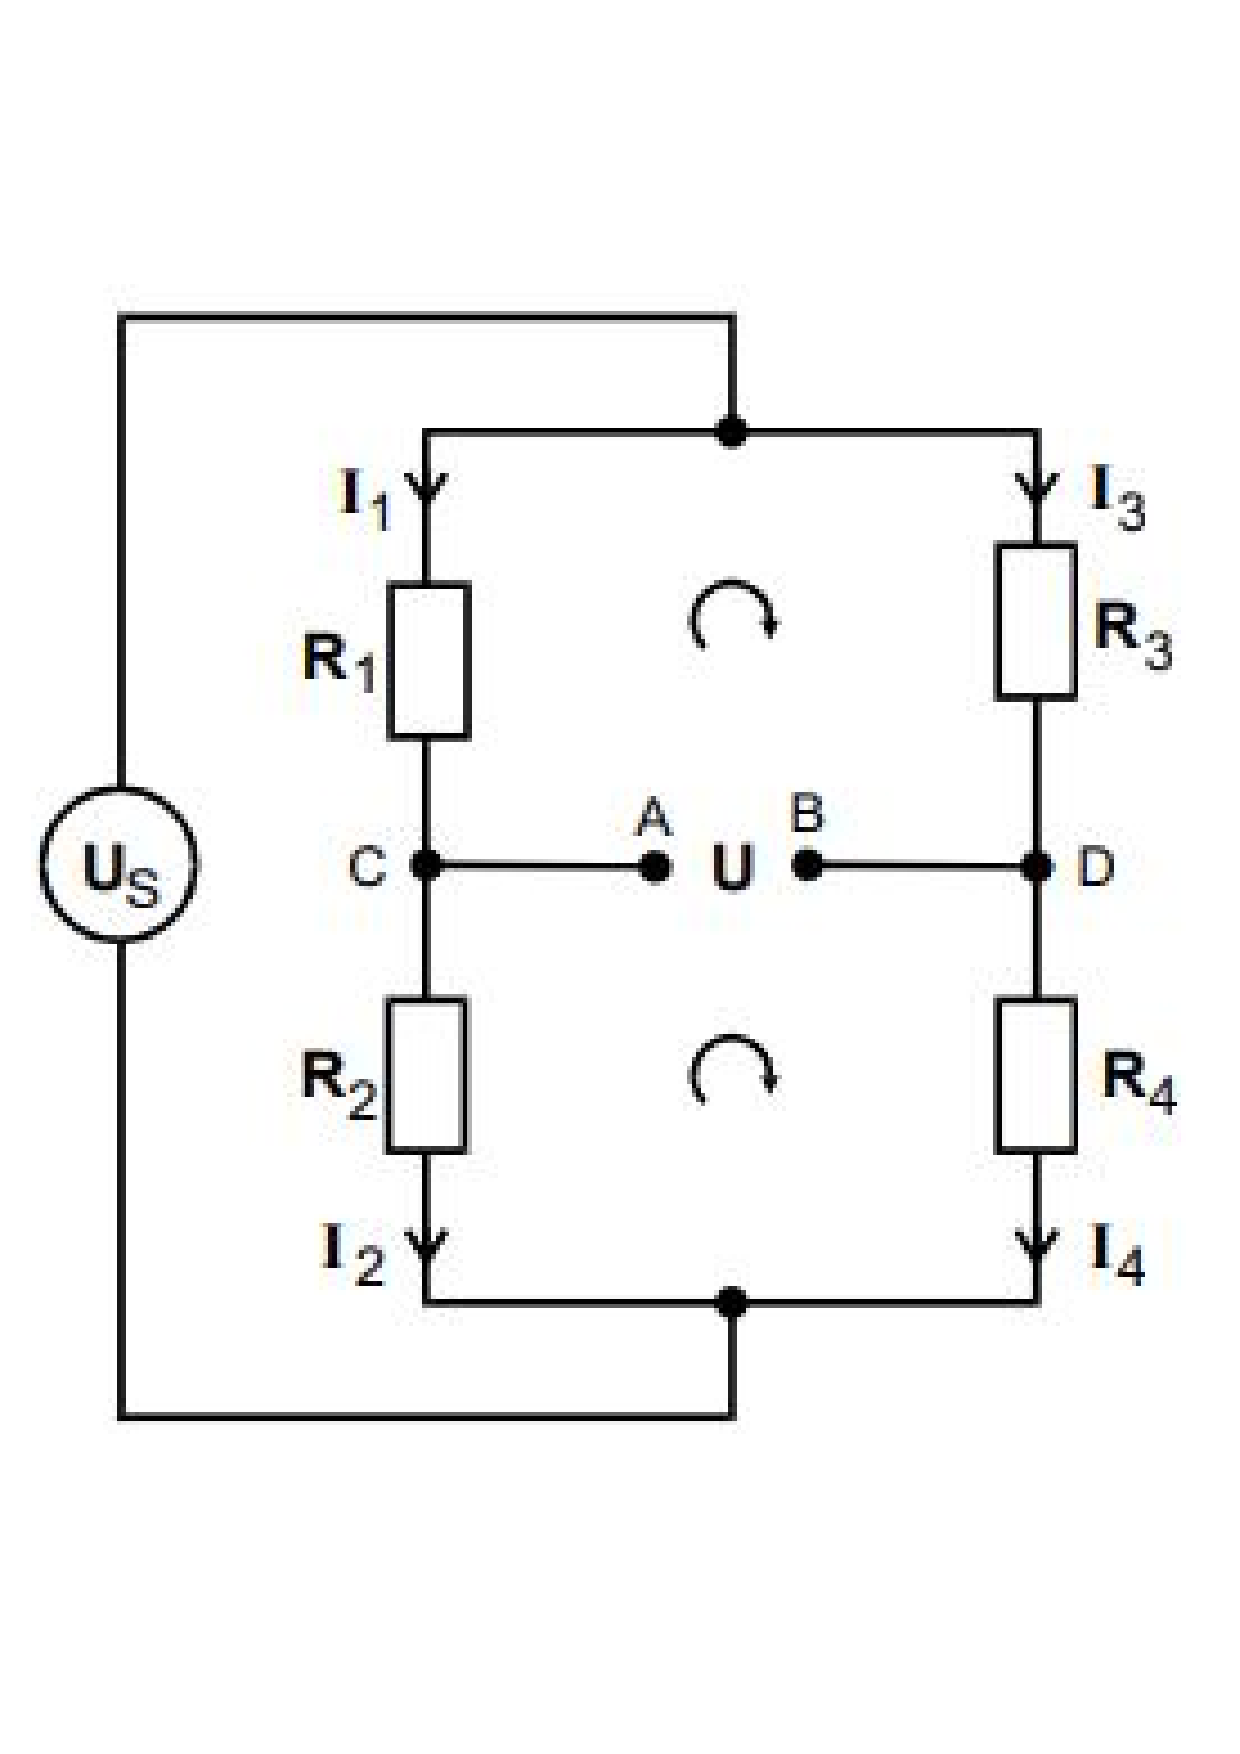
\includegraphics[width=\textwidth]{BrückAllg.pdf}
    \caption{Allgemeiner Aufbau einer Brückenschaltung.\cite{anleitung}}
    \label{fig:Allgemein}
\end{figure}

Allgemein sieht eine Brückenschaltung aus wie in Abbildung \ref{fig:Allgemein}.
Es wird eine Speisespannung angelegt, der Strom teilt sich dann auf zwei getrennten Leitern auf.
In diesem Fall sind an jedem Leiter zwei ohmsche Widerstände angebracht.
An den Punkten A und B wird die sogenannte Brückenspannung abgegriffen.

Mithilfe der Kirchhoffschen Regeln kann die Brückenspannung $U_{AB}$ berechnen.
\begin{enumerate}
    \item {Die Knotenregel
    
    Die Summe aller eintretenden Ströme ($I>0$) ist gleich der Summe aller austretenden Ströme ($I<0$)an einem Knoten.
    \begin{equation}
        {\sum_{i=1}^N I_i} = 0
    \end{equation}
    }

    \item{Die Maschenregel
    
    Die Summe aller Spannungen in einem geschlossenen Stromkreis ist gleich Null.
    \begin{equation}
        {\sum_{i=1}^N U_i} = 0
    \end{equation}}
\end{enumerate}

Daraus folgt:
\begin{equation}
    U = \frac{R_2 \cdot R_3 - R_1 \cdot R_4}{(R_3 + R_4) \cdot (R_1 + R_2)} \cdot U_S .
\end{equation}

Dabei ist $U_S$ die Speisespannung.
Wenn auf beiden Leitern das gleiche Widerstandsverhältnis besteht, verschwindet die Brückenspannung.
Also wenn die folgende Abgleichbedingung gilt:
\begin{equation}
\label{eq:Abgleichbedingung}
    R_1 \cdot R_4 = R_2 \cdot R_3 .
\end{equation}
So eine Brücke wird abgeglichen genannt.
Dies ermöglicht Widerstandsmessungen, bei denen ein Widerstand unbekannt ist.
Durch Variation der bekannten Widerstände bis die Brückenspannung gleich Null ist, kann der unbekannte Widerstand ermittelt werden.

Bei Brückenschaltungen können auch komplexe Widerstände eingebaut werden.
Bei den Formeln muss dann nur noch beachtet werden, dass sich der Widerstand in Blind- und Wirkwiderstand aufteilen lässt.

\subsection{Wheatstonesche Brücke}

Die Wheatstonesche Brücke kann mit Gleich- oder Wechselstrom betrieben werden, da sie nur ohmsche Widerstände enthält. 
Drei davon sind bekannt.
Der unbekannte Widerstand $R_x$ kann durch \eqref{eq:Abgleichbedingung} ermittelt werden, indem die Formel nach $R_x$ umgestellt wird.
$R_1$ wird in diesem Fall durch $R_x$ ersetzt.
\begin{equation}\label{eqn:wheatstone}
    R_x = R_2 \cdot \frac{R_3}{R_4}
\end{equation}
Da $R_x$ vom Verhältnis $R_3$ und $R_4$ abhängt, wird ein Potentiometer verwendet.

\begin{figure}
    \centering
    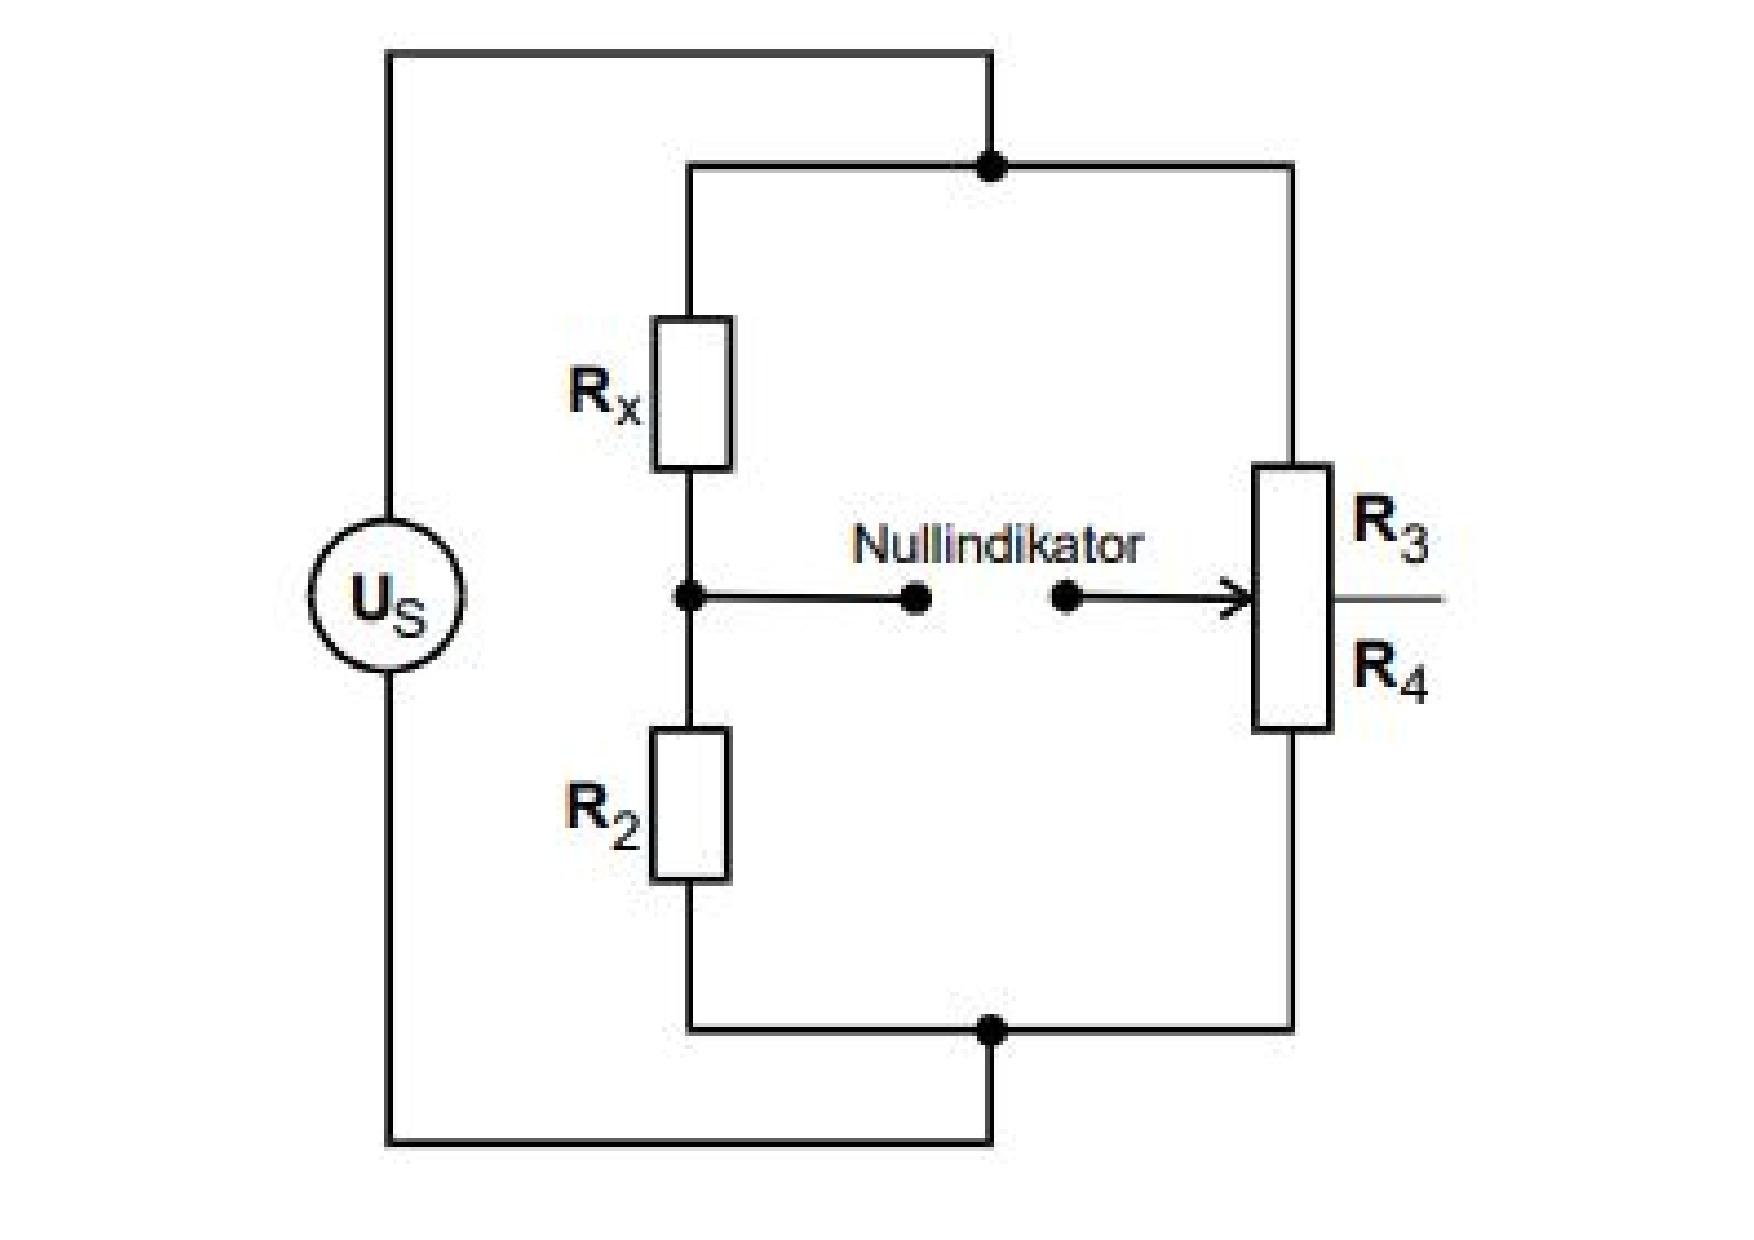
\includegraphics[width=\textwidth]{wheatBruecke.pdf}
    \caption{Aufbau einer Wheatstonesche Brücke.\cite{anleitung}}
\end{figure}

\subsection{Kapazitätsmessbrücke}
\label{sec:Kapazität}

Diese Schaltung wird mit Wechselstrom betrieben, da hier komplexe Widerständne eingebaut werden.
Da ein realer Kondensator einen Teil der elektrischen Energie in Wärme umwandelt, wird dies mit einem Ersatzschaltbild realisiert, indem ein ohmscher Widerstand und eine Kapazität in Reihe geschalten werden.
Um die von $R_x$ verursachte Phasenverschiebung zu kompensierern, wird der ohmsche Widerstand $R_2$ vom zweiten realen Kondensator veränderlich sein.

Es folgt:
\begin{equation} \label{eqn:kapazität1}
    R_x = R_2 \cdot \frac{R_3}{R_4}
\end{equation}
und
\begin{equation} \label{eqn:kapazität2}
    C_x = C_2 \cdot \frac{R_4}{R_3} .
\end{equation}

\begin{figure}
    \centering
    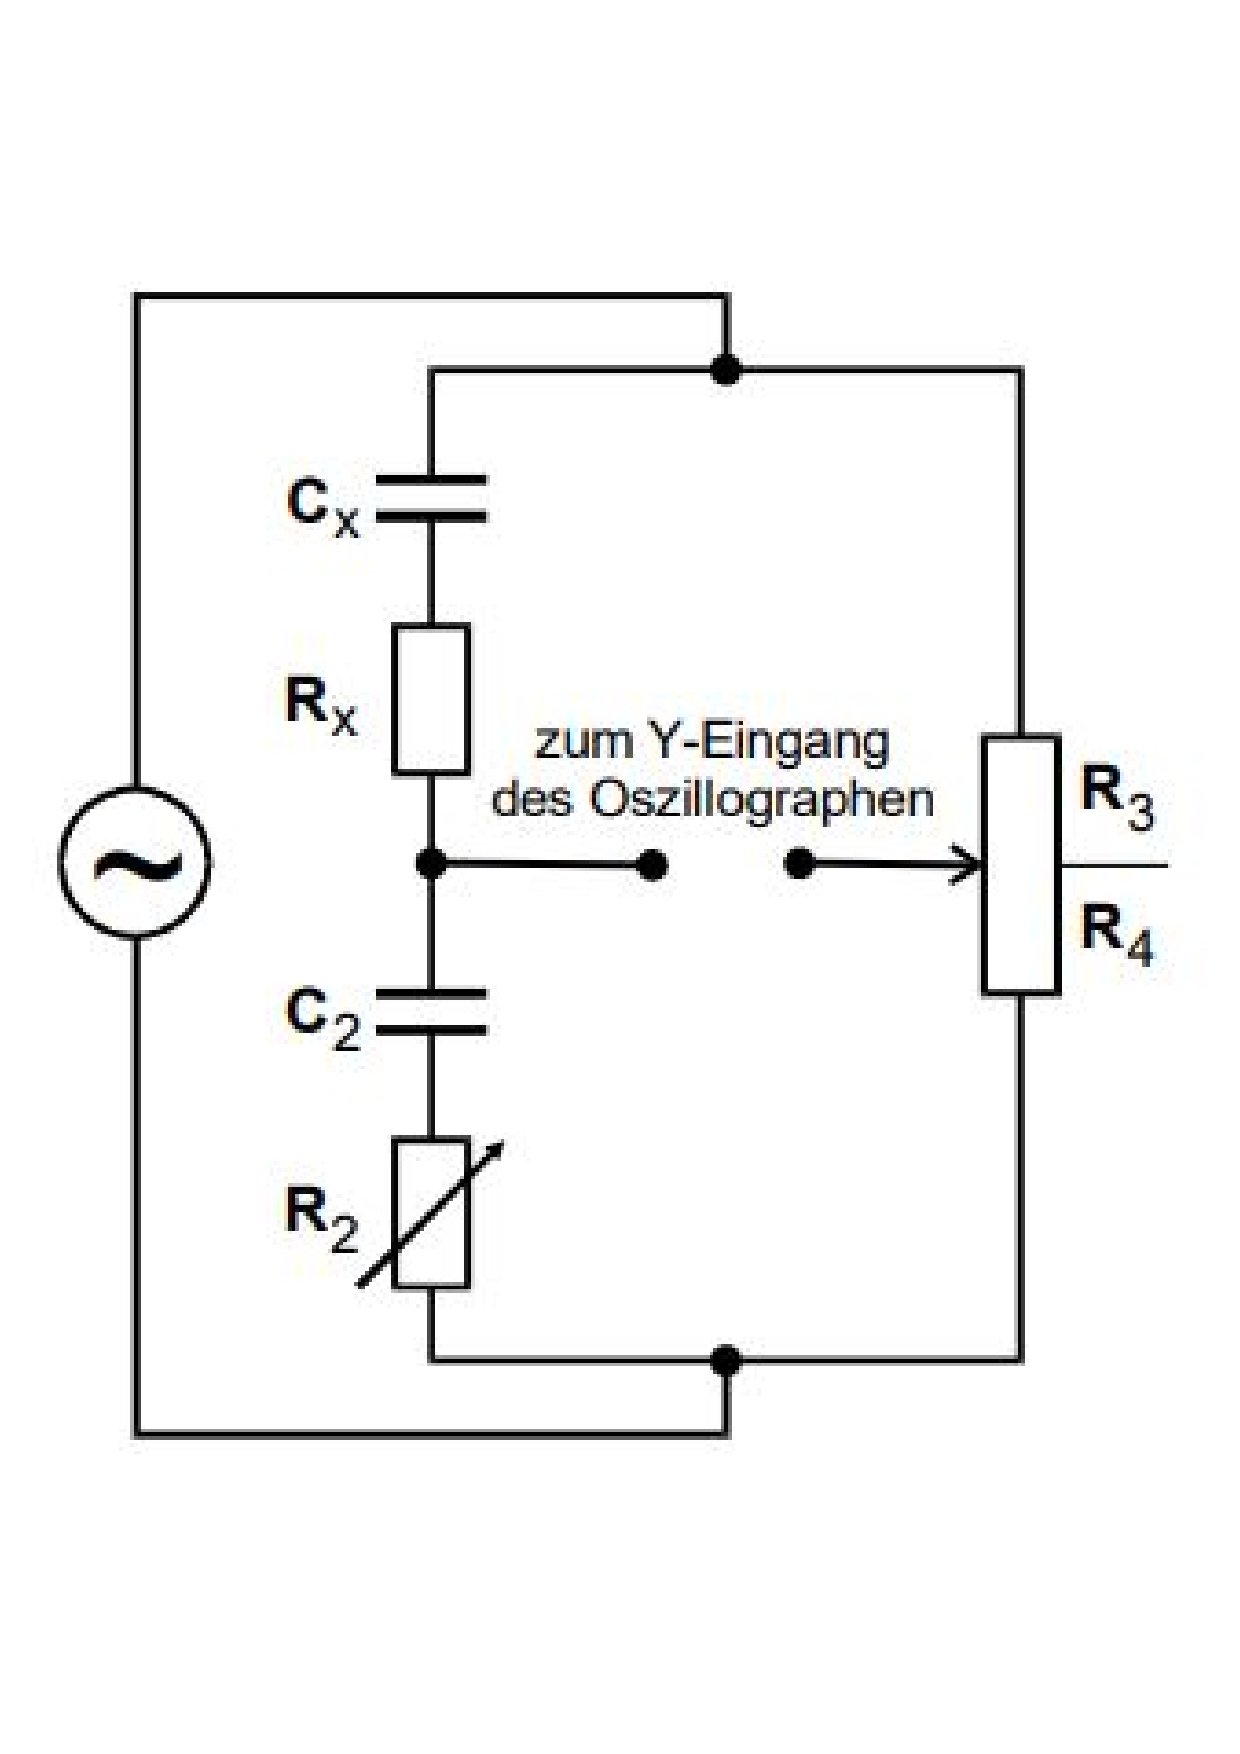
\includegraphics[width=\textwidth]{KapBruecke.pdf}
    \caption{Aufbau einer Kapazitätsmessbrücke mit Ersatzschaltbild realer Kondensatoren.\cite{anleitung}}
\end{figure}

\subsection{Induktivitätsmessbrücke}
\label{sec:Induktivität}

Der Aufbau einer Induktivitätsmessbrücke ist ähnlich wie bei \ref{sec:Kapazität} 
Da reale Induktivitäten einen Teil der magnetischen Feldenergie in Wärme umwandeln, ist auch das Ersatzschaltbild analog zu einem realen Kondensator aufgebaut.
Anstelle eines Kondensators wird eine Induktivität mit einem ohmschen Widerstand in Reihe geschaltet.

Es gilt:
\begin{equation} \label{eqn:induktivität_r}
    R_x = R_2 \cdot \frac{R_3}{R_4}
\end{equation}
und
\begin{equation} \label{eqn:induktivität_l}
    L_x = L_2 \cdot \frac{R_3}{R_4} .
\end{equation}

\begin{figure}
    \centering
    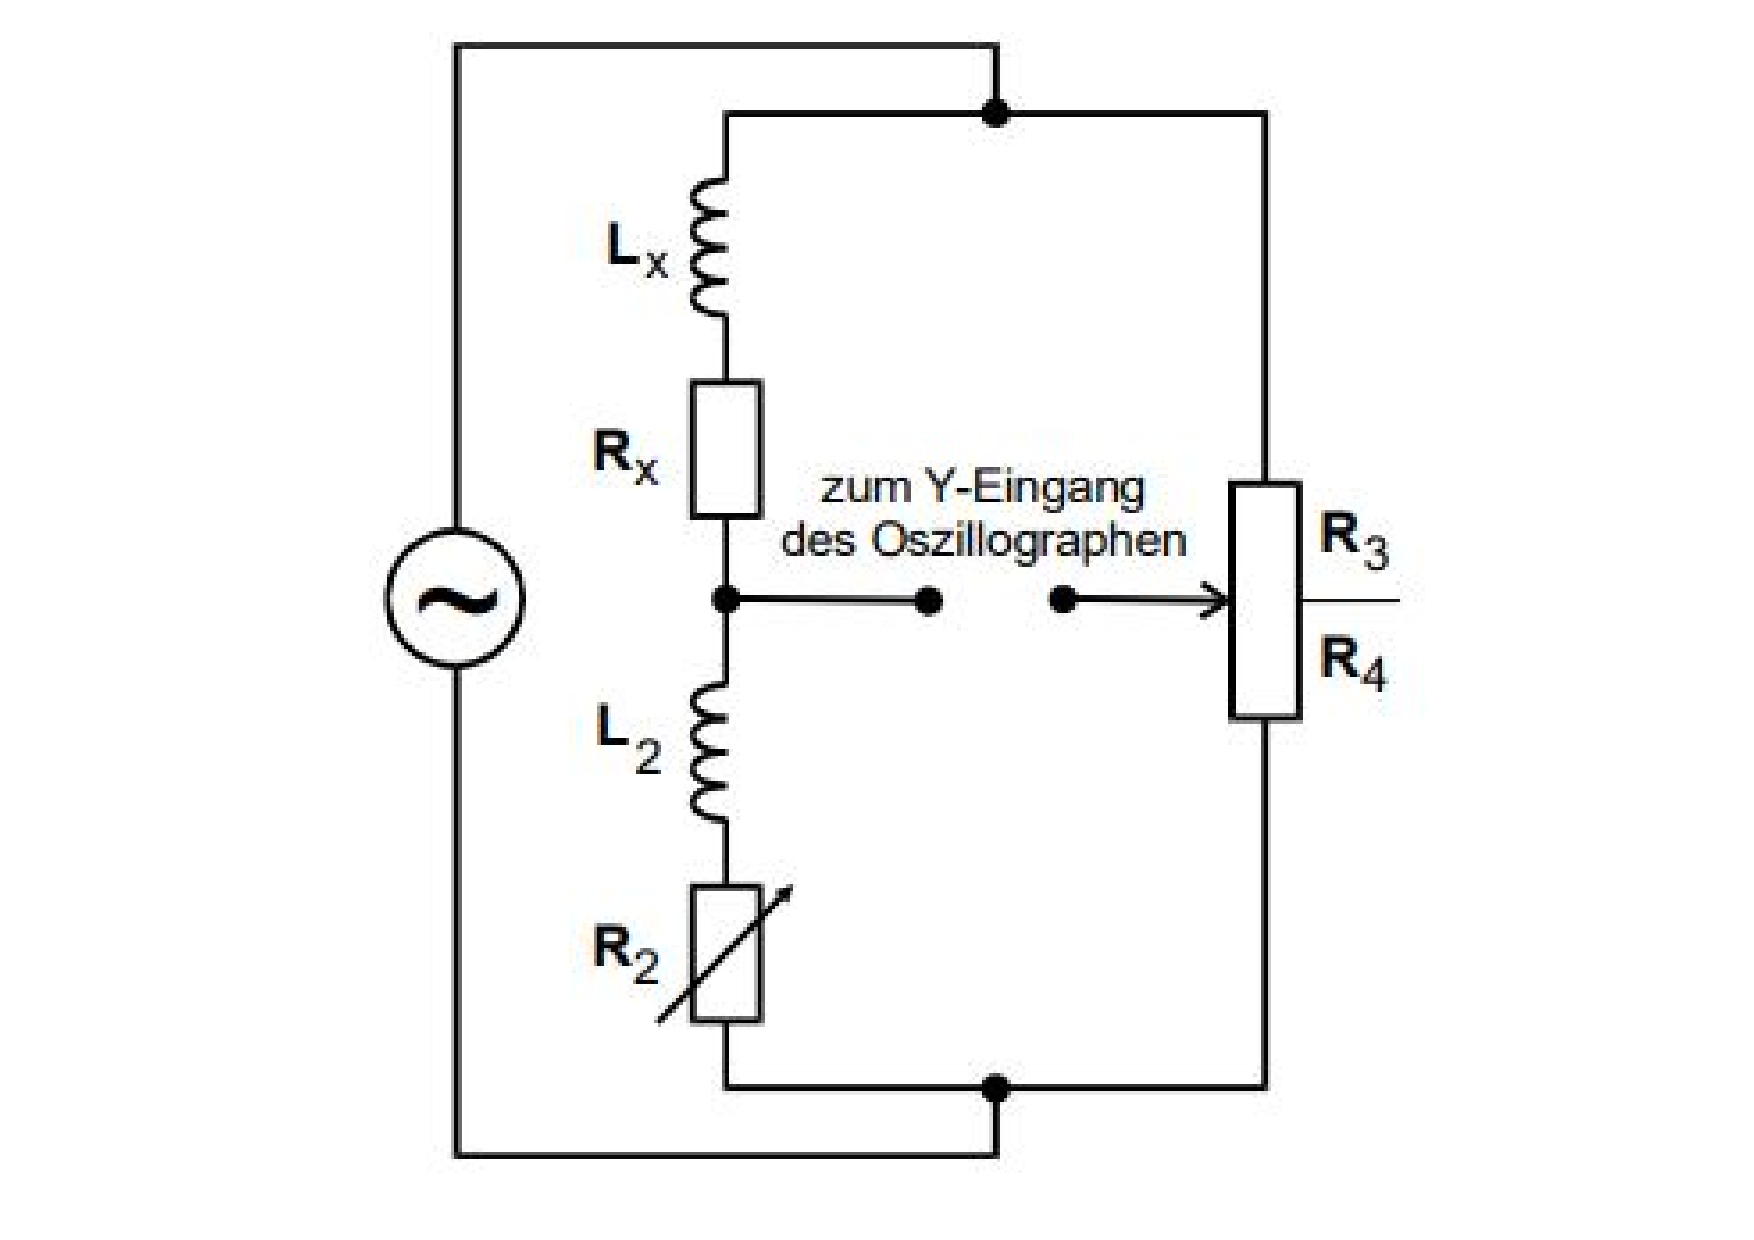
\includegraphics[width=\textwidth]{InduBruecke.pdf}
    \caption{Aufbau einer Induktivitätsmessbrücke mit Ersatzschaltbild realer Induktivitäten. \cite{anleitung}}
    \label{fig:indubruecke}
\end{figure}

Der Wirkanteil der Induktivität $L_2$ soll allein durch $R_2$ verwirklicht werden.
Bei niedrigen Frequenzen ist das schwer umsetzbar.
Eine Induktivitätsmessung mithilfe der Maxwell-Brücke ist eine gute Alternative.

\subsection{Maxwell-Brücke}

\begin{figure}
    \centering
    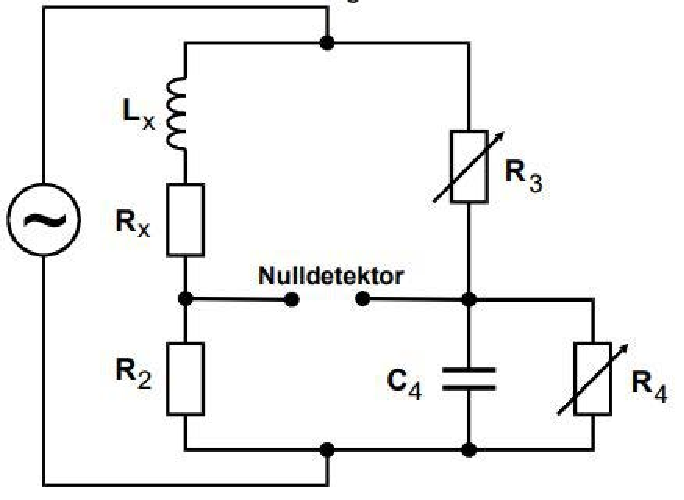
\includegraphics[width=\textwidth]{MaxwellBruecke.pdf}
    \caption{Aufbau einer Maxwell-Brücke. \cite{anleitung}}
    \label{fig:Maxwell}
\end{figure}

Mithilfe der Maxwell-Brücke können auch Induktivitäten ausgemessen werden.
Dabei soll anstelle der Induktivität $L_2$ aus \ref{sec:Induktivität} eine Kapazität verwendet werden.
Diese Kapazität $C_4$ hat einen kleineren Wirkwiderstand und möglichst wenig Verluste.

Der Aufbau dieser Schaltung ist in \ref{fig:Maxwell} abgebildet.

Es gelten folgende Abgleichbedingungen:
\begin{equation}
    R_x = \frac{R_2 \cdot R_3}{R_4}
\end{equation}
und
\begin{equation}
    L_x = R_2 \cdot R_3 \cdot C_4 .
\end{equation}

\subsection{Wien-Robinson-Brücke}

\begin{figure}
    \centering
    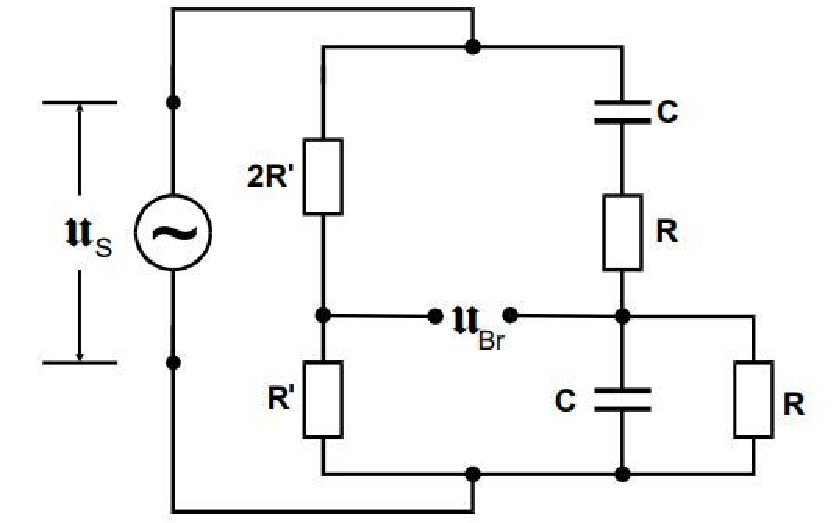
\includegraphics[width=\textwidth]{WienRobinBruecke.pdf}
    \caption{Aufbau einer Wien-Robinson-Brücke. \cite{anleitung}}
\end{figure}

Die Wien-Robinson-Brücke fungiert als ein elektronischer Filter.
Der Abgleich ist hier nur bei einer bestimmten Frequenz $\omega_0$ möglich, umliegende Frequnzen werden abgeschwächt.
Sonstige Abgleichelemente wie bei den vorherigen Brücken sind nicht enthalten.
Die Brückenspannung $U_{Br}$ soll in Abhängigkeit von der Frequenz ermittelt werden.

Für den Betrag des Verhältnisses zwischen Brücken- $U_{Br}$ und Speisespannung $U_S$ gilt:
\begin{equation}
    \label{eq:U_br durch U_s}
    \lvert{\frac{U_{Br}}{U_S}}\rvert^2 = \frac{(\omega^2 \cdot R^2 \cdot C^2 - 1)^2}{9 \cdot \{(1 - \omega^2 \cdot R^2 \cdot C^2)^2 + 9 \cdot \omega^2 \cdot R^2 \cdot C^2\}} .
\end{equation}

Bei 
\begin{equation}
    \omega_0 = \frac{1}{R \cdot C}
\end{equation}
verschwindet die Brückenspannung.
Wird nun
\begin{equation}
    \Omega = \frac{\omega}{\omega_0}
\end{equation}
in \eqref{eq:U_br durch U_s} eingeführt, folgt für das Verhältnis der Spannungen:
\begin{equation}
    \label{eq:Verhältnis U mit Verhältnis omega}
    \lvert{\frac{U_{Br}}{U_S}}\rvert^2 = \frac{1}{9} \cdot \frac{(\Omega^2 - 1)^2}{(1 - \Omega^2)^2 + 9 \cdot \Omega^2} .
\end{equation}
An \eqref{eq:Verhältnis U mit Verhältnis omega} sieht man deutlich, dass Frequenzen in der Nähe von $\omega_0$ auch stark abgeschwächt werden.

Mithilfe der Wien-Robinson-Brücke kann die Qualität eines Sinusgenerators gemessen werden.
Bei der Frequenz $\omega_0$ kommt es zu keiner Brückenspannung.
Dennoch wird etwas gemessen, verantwortlich dafür sind Oberwellen.
Diese sind bei einem realen Sinusgenerator nicht auszuschließen.
Der Klirrfaktor beschreibt das Verhältnis dieser Oberwelle zur Grundwelle einer Sinusschwingung des Generators
und damit die Qualität des Generators.